\begin{enumerate}[label=\thesection.\arabic*.,ref=\thesection.\theenumi]
\numberwithin{equation}{enumi}



\item For the control system shown in \ref{fig:ee18btech11044_1} write the steady state output for step input. \\
\solution
\begin{align}
\lim_{t\to\infty} y(t)  = \lim_{s\to0} sY(s) \\
\lim_{s\to0} sY(s) = \lim_{s\to0}  \frac{s R(s)}{1+G(s)} \\
\lim_{s\to0} sY(s) = \frac{1}{1 + \lim_{s\to0}G(s)}
\end{align}
\begin{figure}[!ht]
	\begin{center}
		\resizebox{\columnwidth}{!}{\tikzstyle{block} = [draw, fill=white, rectangle, 
    minimum height=1cm, minimum width=1cm]
\tikzstyle{sum} = [draw, fill=white, circle, node distance=1cm]
\tikzstyle{input} = [coordinate]
\tikzstyle{output} = [coordinate]
\tikzstyle{pinstyle} = [pin edge={to-,thin,black}]


% The block diagram code is probably more verbose than necessary
\begin{tikzpicture}[auto, node distance=2cm,>=latex']
    % We start by placing the blocks
    \node [input, name=input] {X(s)};
    \node [sum, right of=input] (sum) {};
    
    \node [block, right of=sum] (system) {$G(s)$ };
   
    % We draw an edge between the controller and system block to 
    % calculate the coordinate u. We need it to place the measurement block. 
    
    \node [output, right of=system] (output) {};
    \node [block, below of=system] (measurements) {1};

    % Once the nodes are placed, connecting them is easy. 
    \draw [draw,->] (input) -- node {$R(s)$} (sum);
    \draw [->] (sum) -- node {} (system);
    \draw [->] (system) -- node [name=y] {$Y(s)$}(output);
    \draw [->] (y) |- (measurements);
    \draw [->] (measurements) -| node[pos=0.99] {$-$} 
        node [near end] {} (sum);
\end{tikzpicture}
}
	\end{center}
\caption{}
\label{fig:ee18btech11044_1}
\end{figure}

\item What do you mean by steady state error and write the expression for steady state error for control system shown in \ref{fig:ee18btech11044_1} considering step input. \\
\solution 
Steady-state error is the difference between the input and the output for a prescribed test input as time tends to infinity.
\begin{align}
    e_{ss} = \lim_{s\to0} \frac{1}{1 +G(s)}
\end{align}

\item Refer the definition and calculating phase margin in section 9. \\
\solution 

\item Write the general expression for the transfer function of a phase lead compensator. \\
\solution 
\begin{align}
    G_c(s) =  K_{comp}  \alpha  \frac{(1+\frac{s}{z})}{(1+ \frac{s}{p})} \\
    \alpha = \frac{z}{p}
\end{align}

\begin{figure}[!ht]
	\begin{center}
		\resizebox{\columnwidth}{!}{\tikzstyle{block} = [draw, fill=white, rectangle, 
    minimum height=1cm, minimum width=1cm]
\tikzstyle{sum} = [draw, fill=white, circle, node distance=1cm]
\tikzstyle{input} = [coordinate]
\tikzstyle{output} = [coordinate]
\tikzstyle{pinstyle} = [pin edge={to-,thin,black}]


% The block diagram code is probably more verbose than necessary
\begin{tikzpicture}[auto, node distance=2cm,>=latex']
    % We start by placing the blocks
    \node [input, name=input] {X(s)};
    \node [sum, right of=input] (sum) {};
    
    \node [block, right of=sum] (system) {$G(s)$ };
   
    % We draw an edge between the controller and system block to 
    % calculate the coordinate u. We need it to place the measurement block. 
    
    \node [output, right of=system] (output) {};
    \node [block, below of=system] (measurements) {1};

    % Once the nodes are placed, connecting them is easy. 
    \draw [draw,->] (input) -- node {$R(s)$} (sum);
    \draw [->] (sum) -- node {} (system);
    \draw [->] (system) -- node [name=y] {$Y(s)$}(output);
    \draw [->] (y) |- (measurements);
    \draw [->] (measurements) -| node[pos=0.99] {$-$} 
        node [near end] {} (sum);
\end{tikzpicture}
}
	\end{center}
\caption{}
\label{fig:ee18btech11044_2}
\end{figure}


\item What are the steps involved in designing a lead compensator, explain briefly. \\ 
\solution
\begin{itemize}
    \item Add poles at the origin so that steady state error (generally ramp input is taken) becomes finite.
    \item find the value of $K_{comp}$ from the desired value of steady state error.
    \item Check whether the system satisfies the phase margin criterion.
    \item If not then calculate the additional phase to be added at $w_{gc}$. considering the small change in $w_{gc}$.
    \item Now calculate $\alpha$, z and p as we know the maximum phase and the frequency at which it occurs.
    \item If designed compensator does not satisfy the required criterion then add a bit more phase to compensate for shift in $w_{gc}$.
\end{itemize}


\item For a unity feedback system shown in Fig.1.2, $\frac{K}{s(s+1)}$. Design a lead compensator such that the phase margin of the system is 45$^{\circ}$ and appropriate steady state error is less than or equal to $\frac{1}{15}$ units of the final output value. Further the gain crossover frequency of the system must be less than 7.5rad/sec. \\

\solution 
For the following reasons, i think this problem cannot be solved
\begin{itemize}
    \item Let us find $K_{comp}$ from the desired steady state error(generally step function or ramp function is considered as input).
    \item Using equations 1.1.3 and 1.2.1 steady state value for step input is 1 and steady state error for step input is 0.
    \item As the steady state error is always zero the value of $K_{comp}$ can be anything.
    \item For ramp input, steady state error is finite but steady state value of output is infnity, so no value of $K_{comp}$ can satisfy the desired steady state error condition. 
    \item unique $K_{comp}$ cannot be found which satisfies the desired conditions.
    \item Calculating the phase margin of given system is a necessary step as we would know the phase to be added to achieve the desired phase margin, but phase margin of given system cannot be calculated without the knowledge of K. 
\end{itemize}

\item Plot how phase margin is varying as K is varying  \\ 
\solution
\begin{lstlisting}
codes/ee18btech11044_2.py
\end{lstlisting}

\begin{figure}[!ht]
\centering
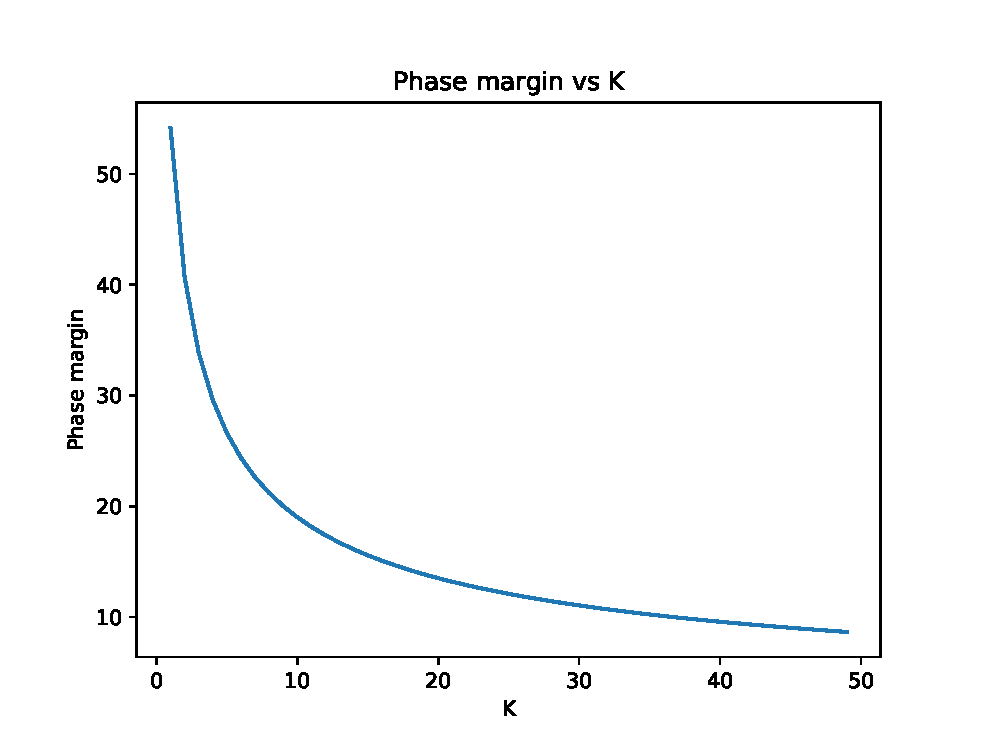
\includegraphics[width=\columnwidth]{./figs/ee18btech11044_2.eps}
\end{figure}

\end{enumerate}
